\documentclass{article}
\usepackage{url}
\usepackage[usenames,dvipsnames]{color}
\usepackage[utf8]{inputenc}
\usepackage{graphicx}%for includegraphics
\graphicspath{ {./images/} }
\usepackage{float}


\title{Report: Atari Breakout with Reinforcement Learning}
\author{ Cecilia Aponte \\ \\
  Sapienza Universita di Roma\\
  Master of Artificial Intelligence and Robotics \\
  AI - Reinforcement Learning\\
}


\begin{document}
\maketitle

\section{Introduction}

Reinforcement Learning is an area in machine learning that through experience, it teaches an agent what actions to take. The actions taken by the agent have to be suitable to maximize the reward in the environment. One environment where Reinforcement Learning can be implemented are games. Breakout from Atari is such a game available as an environment in OpenAI Gym. This report discusses the Reinforcement Learning algorithm and result implementation. The implementation uses Double Q-learning with Deep Convolutional Neural Network. Two different architectures of the CNN are tested also to compare results.

\section{Problem}
In order to solve the Atari Breakout game, the agent has to learn what actions to perform depending on the environment state. The agent has the information of the screen given as pixel information, making it fully observable. Through the pixels, the agent can therefore learn to understand the blocks, and the position of the ball and paddle. With this information about the state, the agent has to predict the action it must take. This way, the agent will achieve the goal to breakout all the blocks and achieve a high score. An example of the game environment is seen in Figure 1. 

\begin{figure}
    \centering
    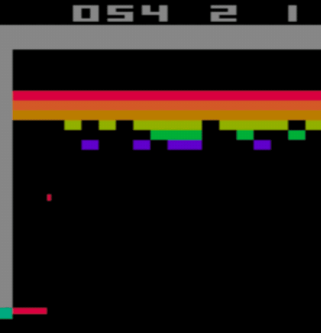
\includegraphics[width=.6\textwidth]{Breakout_Playing.png}\hfill
    \caption{Atari Breakout Environment where the agent has to learn to achieve.} 
\end{figure}


\section{Model}
The movement direction and velocity of the objects in the screen are synthesized by stacking 4 consecutive frames into the network. Each screen image is reduced from RGB to grayscale and cropped to only include the relevant objects (removing the score, etc.). Therefore the image of dimension (210,160,3) is converted to (180,160,4). And a batch size of 64 randomly selected from the memory to get different transitions throughout all the memory. The final structure is reshaped to (4, 180, 160, 64). \\

To learn the actions that the agent must employ, the model is built to both explore and exploit. Initially, the model learns by taking random actions to explore what actions work well under which circumstances. Then with some experience, it will start exploiting the knowledge using the highest q-value. It will build a probability based on the state and previous learned scenarios to select an action with the highest probability and reward. In summary, the approach is to have an agent that is executing actions on the environment, observing the outcomes for those actions, collecting the rewards, and using this reward knowledge to modify future actions to improve its performance. This is seen in the diagram in Figure 2 describing the way the agent interacts with the environment. \\

The agent learns the policy strategy to evaluate and recommend the next action given a specific state. The agent selects the policy that maximizes the future expected reward for a given action, this way it will maximize the overall reward. 


\begin{figure}
    \centering
    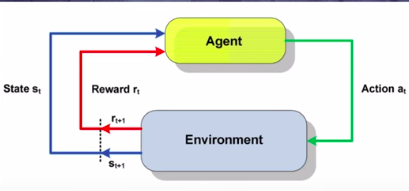
\includegraphics[width=.7\textwidth]{Reinf_Graph.png}\hfill
    \caption{Diagram showing the interaction between the agent and environment.} 
\end{figure}

\subsection{Variables}
There are four important variables used by the agent to learn and reach its goal: states, actions, transitions, and reward. \\

The state is the information regarding the environment. It includes every configuration of the paddles and ball as a state. Every state has a state transition describing how the state will change with a given action, described as a tuple: (state, action, reward, next state, terminal). There are four actions in Breakout: 0: do nothing, 1: fire ball to start game, 2: move right, 3: move left. And every transition has a reward of 0 except for the final terminal state, where the reward may be +1 or -1. 


\subsection{Learning Task}
Q-learning has the goal to learn a policy that decided what action the agent takes under what circumstances. The Q 'quality' is the best score at the end of the game given the chosen action and state. \\
This is given by the policy: \\
\begin{equation}
\pi (s) = argmax_a Q(s,a)
\end{equation}
And Q-function is approximated using the Bellman equation: \\
\begin{equation}
Q(s,a) = r + \gamma \cdot max_{a'} Q(s',a')
\end{equation}

Deep Q-Learning can be used to estimate guesses for states that have not been visited before, since in reality the amount of states is too high to visit all $256^{180 x 160 x4}$. A Neural Network is used to state (pixels of 4 consecutive screens) and an action as input and outputs the corresponding Q-value. Table 1 shows the convolutional neural network used with three convolutional layers, followed by two fully connected layers.

\begin{table}[ht]
    \centering
    \begin{tabular}{||c c c c c c||} 
     \hline
     Layer & Input & Filter Size & Stride & Num Filters & Activation \\ [0.5ex] 
     \hline\hline
     conv1 & 180x160x4 & 8x8 & 4 & 32 & ReLU \\ 
     \hline
     conv2 & conv1 output & 4x4 & 2 & 64 & ReLU \\
     \hline
     conv3 & conv2 output & 3x3 & 1 & 64 & ReLU \\
     \hline
     fc4 & conv3 output & & & 512 & ReLU \\
     \hline
     fc5 & fc4 output & & & 4 & Linear \\ [1ex] 
     \hline
    \end{tabular}
    \caption{Convolutional Neural Network Architecture}
    \label{tab:my_label}
\end{table}

The output Q-values can be optimized using squared error loss as seen in Figure 
\begin{figure}[ht]
    \centering
    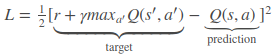
\includegraphics[width=.5\textwidth]{Loss_function.png}\hfill
    \caption{Squared Error Loss used to optimize the output Q-values.} 
\end{figure}

The parameters chosen to train the network are as follows: 
\begin{enumerate}
    \item Learning rate ($\alpha$): To learn slowly by taking small steps in the direction of descent, $\alpha$ is set to 0.005.
    \item Epsilon ($\epsilon$): To explore initially, $\epsilon$ is set to 1.0 until 40k steps are acquired. Then, it decreases linearly by 0.0001 until it reaches 0.01 where it stays the rest of the training.
    \item Gamma ($\gamma$): To balance between immediate and future rewards, the discount factor is set to $\gamma$=0.9. 
\end{enumerate}

During the training process, the agent chooses the action and this results in observing the reward and next step. This transition to the net step is given as a tuple as $(state, action, reward, next state, terminal)$. This is stored in memory, where the 50k most resent transition are stored as well. This way, during training a batch of 64 random samples from this memory are used instead of the most recent transition so that subsequent samples are not similar and thus driving the network to a minimum. \\

The rewards assigned after an action is selected for a state is given by Atari as 0 or 1. In order to improve the results, reward discounting was introduced by adding another reward value of -1 when the agent does not succeed and has no more lives. This way, the algorithm is encouraged by positive rewards and discouraged by negative ones. \\

Lastly, a Double Q-Learning (DDQN) algorithm is used to improve the network. This method is used to overcome overestimation of actions in noisy environments, since when this happens it become harder for the agent to explore equally to find the right policy. The DDQN solves this by decoupling the network into two, one to select an action and the other as a target network to generate the Q-value for the action chosen. The separate formulas are given by Figure 4.

\begin{figure}[ht]
    \centering
    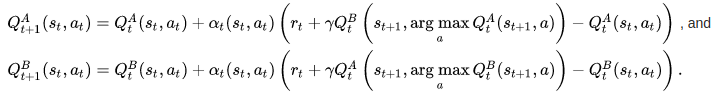
\includegraphics[width=1\textwidth]{DDQL_function.png}\hfill
    \caption{Double Q-Learning formulas for the separate networks.} 
\end{figure}



\section{Solution}
Three different algorithms were implemented to test and compare the results. Those are:
\begin{enumerate}
    \item Algorithm I: 3 CNN layers with conv3 layer using 128 filters and fc4 layer using filter size 256. Uses 3 actions.
    \item Algorithm II: 3 CNN layers with conv3 layer using 64 filters and fc4 layer using filter size 512. Uses 4 actions, included 'do nothing' action. And discounted reward of -1 when agent dies.
    \item Algorithm III: Longer exploration (40k instead of 25k) and higher learning rate (0.005 instead of 0.0002), fc5 layer changed from ReLU to linear activation, and gamma from 0.99 to 0.9. This last implementation was described throughout this report.
\end{enumerate}


\section{Evaluation and Discussion of Results}
The series of algorithm that were tested improved in the order they are shown. Each training run results gave clues as to what changes were necessary to improve the network. 

\begin{enumerate}
    \item Algorithm I: As seen in Figure 5, algorithm I which was run for 2,000 games shows a learning where the scores oscillate between 0 and 8. Higher scores are seen near the exploration phase as seen by epsilon that starts and stays at 1 until it decreases linearly as expected. Reward stays at 0, since no wins were seen during training. 
    
    \begin{figure}[H]
    \centering
    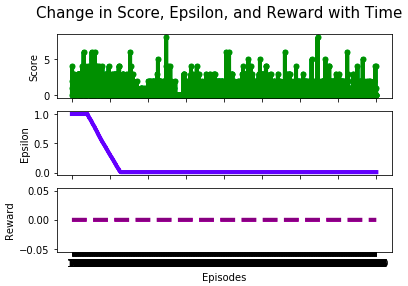
\includegraphics[width=0.8\textwidth]{Results_01.png}\hfill
    \caption{Score, Reward, and Epsilon results using the first algorithm.} 
\end{figure}
    
    \item Algorithm II: As seen in Figure 6, the score again oscillates during training. Reaching a maximum value of 6 and minimum of -1. The average score is between -0.4 and 1, which a third-degree polynomial function drawn to show the trend of the training. Based on that, there seems to be an increase in the average score if training would continue longer.
    
    \begin{figure}[H]
        \centering
        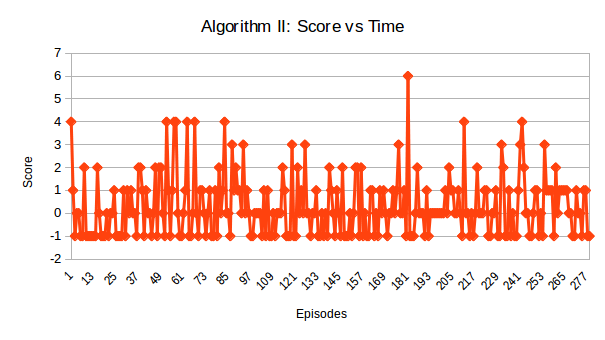
\includegraphics[width=.8\textwidth]{Algorithm2_score.png}\hfill
        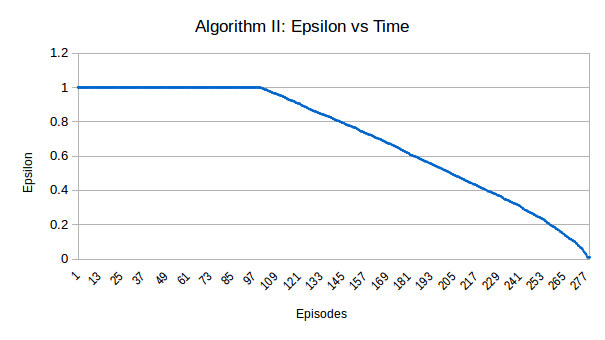
\includegraphics[width=.8\textwidth]{Algorithm2_epsilon.png}\hfill 
        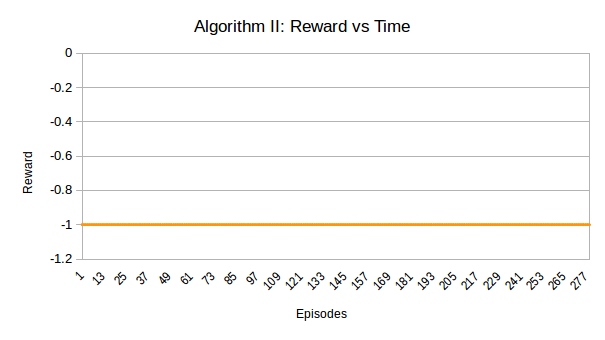
\includegraphics[width=.8\textwidth]{Algorithm2_reward.png}\hfill 
        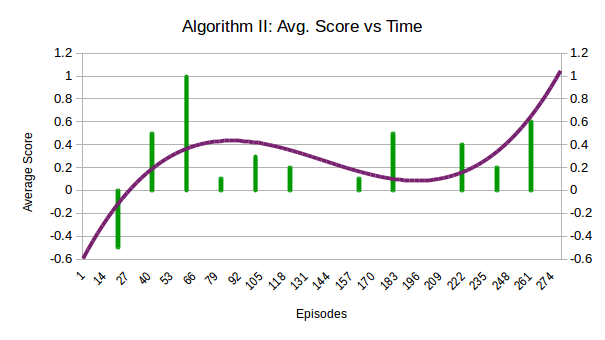
\includegraphics[width=.8\textwidth]{Algorithm2_Avgscore.png}\hfill 
        \caption{Score, Reward, and Epsilon results using the second algorithm.}
    \end{figure}
    
    \item Algorithm III: This third implementation shows an overall higher score. There are more values at 2 or higher as seen in Figure 7. The average of the data is 0.62 and median 1, while Algorithm II is 0.3 and 0, respectively. The Average Score shows that during the last 200 episodes, it has a higher score compared to all algorithms and even the beginning of the same algorithm III (1.1 average, and 1.2 median). If the trend would continue with more training time, the algorithm seems to be capable of converging to a good optimized network.  
    
    
    \begin{figure}[H]
        \centering
        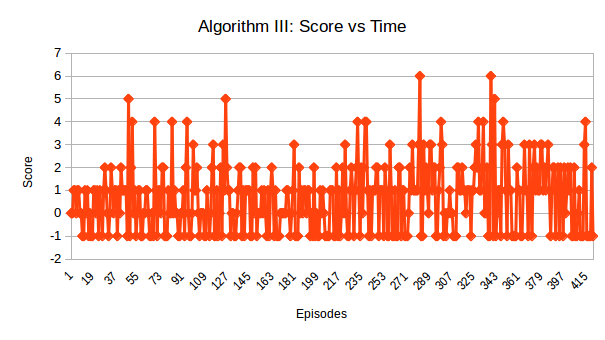
\includegraphics[width=.8\textwidth]{Algorithm3_score.png}\hfill
        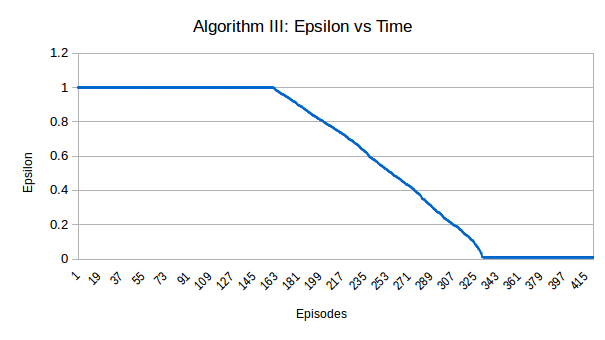
\includegraphics[width=.8\textwidth]{Algorithm3_epsilon.png}\hfill 
        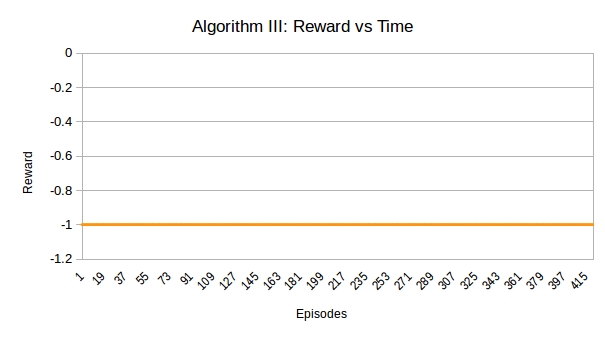
\includegraphics[width=.8\textwidth]{Algorithm3_reward.png}\hfill 
        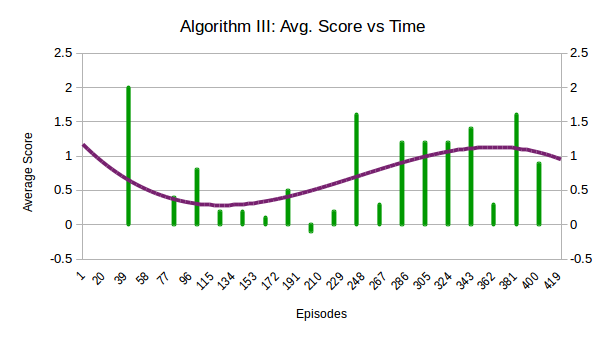
\includegraphics[width=.8\textwidth]{Algorithm3_Avgscore.png}\hfill 
        \caption{Score, Reward, and Epsilon results using the third algorithm.}
    \end{figure}
    
    As the results show, the last algorithm shows promising results. With more training time, the network would be capable of arriving to the optimal agent structure. Another change that would be useful for the algorithm would be to train the network more time with random actions. This would enable a wider range of knowledge about certain actions and states.
    
\end{enumerate}

\section{Conclusion}
The three algorithms implemented show an improvement as the architecture becomes more robust and similar to the algorithm created by Deep Mind. The third algorithm shows a positive outlook with a longer training time, for both exploration and exploitation. \\

Another improvement that could be implemented is the implementation of checkpoints during training so that it can be visualized through Tensorboard and the results captures both visually and as values for future training, if necessary. 




\end{document}




